\documentclass{ceurart}
% Full-paper version of the manuscript; see README.md for build and review status.
% No class, page-geometry or body-font overrides are applied to the CEURART build.
\usepackage{listings}
\usepackage{tabularx}
\usepackage{booktabs}
\usepackage{tikz}
\usetikzlibrary{arrows.meta,positioning}
\usepackage{xurl}
\newcommand{\term}[1]{\texttt{#1}}
\lstset{basicstyle=\small\ttfamily,breaklines=true,columns=fullflexible,
  keepspaces=true,showstringspaces=false,frame=single,
  aboveskip=6pt,belowskip=6pt}
\emergencystretch=1em
\begin{document}

\copyrightyear{2027}
\copyrightclause{Copyright for this paper by its authors.
  Use permitted under Creative Commons License Attribution 4.0
  International (CC BY 4.0).}
\conference{SWAT4HCLS 2027, February 1--4, 2027, Basel, Switzerland}

\title{VCF Core: A Semantic Foundation for RDF Representations of VCF}

\author[1,2]{Elias Crum}[
orcid=0009-0005-3991-754X,
email=elias.crum@ugent.be
]
\cormark[1]
\author[2]{Bart Buelens}[
orcid=0000-0001-7734-3747,
email=bart.buelens@vito.be
]
\author[2]{Gökhan Ertaylan}[
orcid=0000-0001-5602-6435,
email=gokhan.ertaylan@vito.be
]
\author[1]{Ruben Taelman}[
orcid=0000-0001-5118-256X,
email=ruben.taelman@ugent.be
]
\address[1]{IDLab, Department of Electronics and Information Systems, Ghent University -- imec, Belgium}
\address[2]{Flemish institute for Technological Research (VITO) Mol, Belgium}
\cortext[1]{Corresponding author.}



% REVISED: abstract follows context, need, contribution, findings and prospects.
\begin{abstract}
Medical applications of genomic data depend on connecting variant observations to clinical information and biomedical knowledge. 
Linked Data offers a framework for this integration, but the Variant Call Format (VCF) does not natively provide an RDF representation of the observations and their interpretation context. 
We present VCF Core Vocabulary 2.1.1, a shared semantic target for representing VCF files, header declarations, records, annotations and sample data. The vocabulary integrates existing provenance and genomic models while retaining VCF-specific field definitions, ordering and missingness. 
Expanded sample calls expose individual values, whereas condensed, sample-ordered vectors provide an alternative for cohort data. 
Version-specific registries and validation profiles address VCF 4.1--4.5, including 122 reserved INFO and FORMAT declarations for VCF 4.5. 
A curated assessment records representation evidence for all 104 inventoried logical-model constructs and enforcement evidence for 87. 
A complementary specification-derived assessment identifies remaining validation and evidence gaps, distinguishing broad representation coverage from complete conformance. 
A set of 123 curated alignments documents connections to existing variation models and reference ontologies. 
Together, these contributions extend a VCF-to-RDF foundation beyond selected variant attributes while building on earlier semantic representation work. 
We discuss how this foundation could support reusable conversion engines, traceable links to biomedical resources, and SPARQL queries combining genomic observations with medically relevant information.
\end{abstract}
\begin{keywords}
Variant Call Format\sep RDF\sep Genomic data\sep Vocabulary\sep Data integration\sep SHACL
\end{keywords}
\maketitle

% REVISED: motivation before technical detail; no first-ever conversion claim.
\section{Introduction}

Genomic data are increasingly useful in medicine when integrated with other pateint, public, and/or proprietary information. 
A drug-response assessment, for example, depends on the relationship between a patient's genomic findings, a prescribed medication, and the knowledge used to interpret that relationship~\cite{lee2022cpic}.
The presence of a variant alone does not establish these connections. 
Semantic approaches provide a basis for making such connections explicit: HERO-Genomics addresses integration of genomic and biomedical information, while Semantic Beacons demonstrates federated queries over variant data and public knowledge graphs~\cite{cazzaro2025hero,bodrug2025semantic}. 
The maturing investigations of genomic-medical data integration motivates a reusable representation of the source observations on which interpretation depends.

The Variant Call Format (VCF) is widely used to exchange genomic variant data~\cite{danecek2011vcf}. 
It already supports database identifiers, reference information and extensible annotations, so its limitation is not that data linking is impossible. 
Rather, VCF does not natively expose these elements and their relationships in a Findable, Accessible, Interoperable and Reusable (FAIR) way. 
Moreover, a value in a VCF file often depends on a header declaration, an ordered allele list, or the structure of a sample column for its interpretation~\cite{vcf45}. 
Converting only selected variant attributes can leave those dependencies implicit.
Thus, leveraging semantic approaches, such as data modeling using Linked Data and the Resource Description Framework (RDF), is an attractive approach to capturing the full context of information contained within VCF files.

Existing VCF-to-RDF approaches provide important foundations. 
The Genomic Feature and Variation Ontology (GFVO) includes VCF term coverage within a broader model of genomic features and variation, and VCF2RDF presents an isomorphic semantic mapping of the VCF format~\cite{baran2015gfvo,penha2017vcf2rdf}. 
The next step is therefore not to establish that VCF can be represented in RDF. 
It is to provide a shared, version-aware target that combines broad coverage of the source format with explicit connections to these existing models. 
Such a target would allow conversion and querying approaches to develop without each introducing its own interpretation of VCF structure.

Here, we present the VCF Core Vocabulary (\textit{vcfcv}) 2.1.1~\cite{vcfc210}, developed from our earlier VCF-RDFizer Vocabulary~\cite{crum2025semantifying}. 
The contribution combines source-context preservation, alternative sample representations, documented alignment, and coverage evidence across VCF 4.1--4.5. 
After introducing VCF and the model, we explain its relationship to existing work, assess its scope, and discuss how our vocabulary facilitates integrated, medically-relevant genomic querying. 
Throughout, \term{vcfc:} denotes \url{https://w3id.org/vcf-core/vocab#}.

% VCF introduction for readers who already understand RDF and vocabularies.
\section{VCF as a semantic representation problem}
\label{sec:vcf}

\subsection{What a VCF file describes}

A VCF file contains meta-information lines, a column-header line and data records. 
Meta-information lines beginning with \term{\#\#} identify the format version and can describe the reference sequence, genomic sequence segments called contigs, and the fields used in the records. 
The column header begins with \term{\#CHROM}. 
Each subsequent record describes a genomic position, the reference sequence at that position and one or more alternatives, together with observations and annotations~\cite{vcf45}. 
Table~\ref{tab:vcf} summarizes the main components.

\begin{table}[htbp]
\caption{VCF components and the interpretation context that an RDF representation needs to retain. INFO describes a record; FORMAT describes the contents of sample columns.}
\label{tab:vcf}
\centering\small
\begin{tabularx}{\linewidth}{@{}p{0.23\linewidth}X@{}}
\toprule
Component & Role in the source file \\
\midrule
Header declarations & Define field identifiers, types, cardinalities and descriptions, together with reference and processing context. \\
CHROM, POS, ID & Identify the reference contig, position and optional record identifiers. Position alone is not a globally unique variant identifier. \\
REF, ALT & Give the reference allele and ordered alternative alleles. An allele is a sequence alternative at the represented locus. \\
QUAL, FILTER, INFO & Describe call quality, filter status and record-level annotations, including producer-defined fields. \\
FORMAT and samples & Declare an ordered set of keys and give corresponding values for each sample, such as genotype (GT) and read depth (DP). \\
\bottomrule
\end{tabularx}
\end{table}

For example, consider the supplied synthetic record at position 100 on contig 1, with reference allele A, alternative allele G and \term{FORMAT=GT:DP}. 
Its three sample values are \term{0/1:42}, \term{0/0:18} and \term{./.:.}. 
In this biallelic example, genotype \term{0/1} refers to one reference and one alternative allele, while \term{0/0} refers to two reference alleles. 
The values 42 and 18 are read depths. 
The third sample has missing genotype and depth values. 
The slash separates unphased allele calls; a vertical bar is used for phased calls, where the ordering of alleles is meaningful~\cite{vcf45}.

These compact encodings illustrate why representing VCF requires more than assigning predicates to columns. 
Genotype indices refer to the record's ordered allele list, and the meaning of a sample value depends on its FORMAT key. 
Likewise, a header's \term{Number=A} means one value per alternative allele, whereas \term{Number=R} includes the reference allele and \term{Number=G} depends on possible genotypes. 
The same key, such as DP, can occur in INFO and FORMAT without identifying the same observation~\cite{vcf45}.

\subsection{Why version and source context matter}

VCF 4.1--4.5 share these basic structures but differ in supported declarations and constraints~\cite{htsspecs,vcf45}. 
For example, CIPOS describes uncertainty around a reported position. 
Its declared cardinality changes from two values in VCF 4.1--4.3 to two per alternative allele in 4.4--4.5. 
VCF 4.5 also introduces local-allele cardinalities and base-modification fields. 
A common RDF model should support these developments without interpreting an older file under rules introduced later.

A source observation must also remain distinguishable from its biological interpretation. 
Two files may describe the same alteration with different quality scores or annotations. 
A sample column may represent a patient specimen, a pooled sample or a synthetic example. 
Neither records nor sample columns should therefore automatically be equated with normalized variants or patients.

\section{The VCF Core vocabulary}
\label{sec:design}

\subsection{Retaining observations and their provenance}

VCF Core separates a \term{VCFFile}, its \term{VCFHeader}, individual \term{VCFRecord} resources and a \term{VariantCall} associated with each record. 
The call groups quality, filter, annotation and genotype information; it is a modeling abstraction rather than an additional line in the source file. 
Figure~\ref{fig:model} shows this shared structure and the two sample representations.

The file specializes \term{dcat:Distribution} and \term{prov:Entity}, while records and calls provide further attachment points for provenance~\cite{prov2013,vcfc210}. 
File-based IRI templates preserve the relationship between source, record and field. 
Because a VCF identifier can be missing or non-unique, a producer must use a record identifier that distinguishes rows within the source. 
This approach allows observations from different files to remain separate even after they have been linked to a common biological entity.

The property \term{asSequenceAlteration} connects a record or call to a separately described Sequence Ontology (SO) sequence alteration~\cite{eilbeck2005so}. 
FALDO supplies location, reference and position descriptions, including uncertain positions where appropriate~\cite{bolleman2016faldo}. 
Thus, VCF Core does not introduce a competing general-purpose location model. 
Establishing cross-file links still requires compatible reference sequences and correct allele interpretation; the vocabulary provides the connection points rather than a normalization algorithm.

\begin{figure}[htbp]
\centering
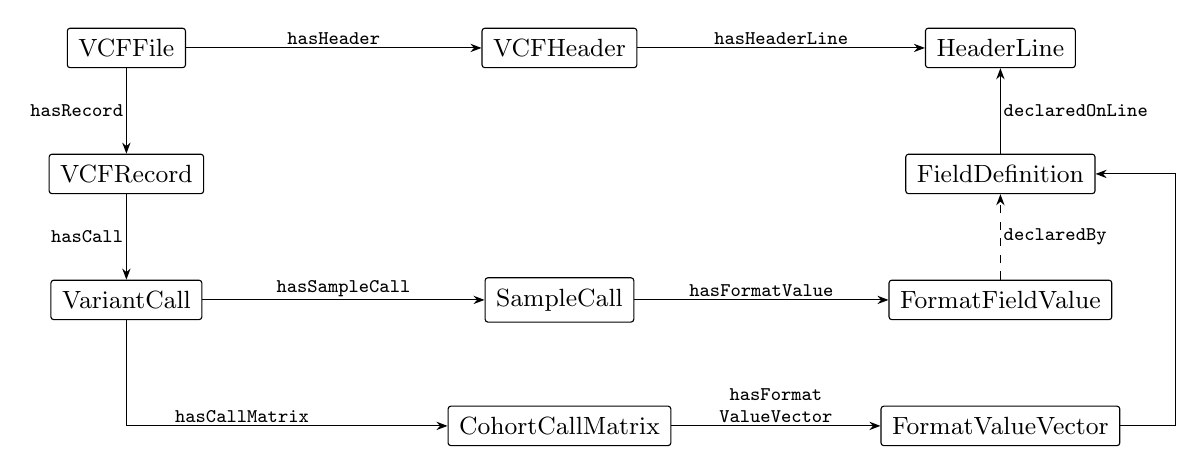
\begin{tikzpicture}[x=1mm,y=1mm,
  box/.style={draw,rounded corners=1pt,align=center,font=\small,inner sep=4pt},
  edge/.style={-{Stealth[length=4pt]},thin},
  lab/.style={font=\scriptsize\ttfamily,fill=white,inner sep=1pt,align=center}]
\node[box] (file) at (17,0) {VCFFile};
\node[box] (header) at (72,0) {VCFHeader};
\node[box] (line) at (128,0) {HeaderLine};
\node[box] (record) at (17,-16) {VCFRecord};
\node[box] (call) at (17,-32) {VariantCall};
\node[box] (definition) at (128,-16) {FieldDefinition};
\node[box] (sample) at (72,-32) {SampleCall};
\node[box] (value) at (128,-32) {FormatFieldValue};
\node[box] (matrix) at (72,-48) {CohortCallMatrix};
\node[box] (vector) at (128,-48) {FormatValueVector};
\draw[edge] (file) -- node[lab,above] {hasHeader} (header);
\draw[edge] (header) -- node[lab,above] {hasHeaderLine} (line);
\draw[edge] (file) -- node[lab,left] {hasRecord} (record);
\draw[edge] (record) -- node[lab,left] {hasCall} (call);
\draw[edge] (definition) -- node[lab,right] {declaredOnLine} (line);
\draw[edge] (call) -- node[lab,above] {hasSampleCall} (sample);
\draw[edge] (sample) -- node[lab,above] {hasFormatValue} (value);
\draw[edge] (call.south) |- node[lab,above,pos=0.68] {hasCallMatrix} (matrix);
\draw[edge] (matrix) -- node[lab,above] {hasFormat\\ValueVector} (vector);
\draw[edge,dashed] (value) -- node[lab,right] {declaredBy} (definition);
\draw[edge] (vector.east) -- ++(7,0) |- (definition.east);
\end{tikzpicture}
\caption{Selected VCF Core relationships; prefixes are omitted. Both sample profiles retain the file, record and header context. 
An expanded value can link to its definition through \term{declaredBy}; the equivalent relation is required for a condensed vector. 
Sample identity and ordering are described separately through \term{VCFSample} and \term{SampleSet}.}
\label{fig:model}
\end{figure}

\subsection{Making field interpretation explicit}

% TODO: This is all descriptive but uninteresting to a general audience, reads more like a Vocab Specification...

Header declarations are represented because they determine how values should be read. 
The vcfcv model includes dedicated classes for the eleven meta-information line types identified in the VCF 4.5 inventory, together with the column-header line. 
Generic \term{HeaderAttribute} resources retain attributes of structured declarations, including producer-defined additions. 
Field definitions expose their identifier, Number, Type, Description and optional source and version information~\cite{vcfc210}.

A standardized field definition and its occurrence in a file have different roles. 
The reserved FORMAT/DP definition describes a key supplied by the specification; a particular header line records what one file declares. 
VCF Core therefore provides distinct \term{FieldDefinition} and \term{HeaderLine} resources, connected by \term{declaredOnLine}. 
Values can refer to their defining declaration through \term{declaredBy}. 
This pattern supports reuse of existing declarations without treating a registry entry as a line present in every file.

Lexical and parsed values are complementary. 
\term{fieldValue} retains a source token or list, while optional integer, decimal and boolean properties support suitable scalar queries. 
A missing depth is not converted to zero, and a non-finite floating-point token is not forced into \term{xsd:decimal}. 
Standalone missing values can use \term{vcfc:Null}; genotype strings retain their allele separators. 
Ordered allele resources use index zero for REF and positive indices for ALT, preserving the context needed to interpret genotype indices and allele-dependent annotations. 
Optional raw fields preserve additional source text, but retaining a string alone is not counted as structured coverage.

\subsection{Choosing how sample data are represented}
\label{sec:profiles}

The expanded profile connects each call to per-sample \term{SampleCall} resources and individual \term{FormatFieldValue} resources. 
This makes values directly accessible through graph patterns and allows an application to annotate a particular sample observation. 
A \term{VCFSample} identifies the source column; linking it to a biological specimen or patient is a separate integration task. 
Expanded representation is applicable to both single- and multi-sample files when direct access justifies the additional graph structure.

Condensed representation associates each call with a cohort matrix. 
The \term{CohortCallMatrix} groups one \term{FormatValueVector} for each represented FORMAT key. 
A shared \term{SampleSet} identifies samples by name and one-based index. 
Each vector specifies its definition, encoding and payload. 
The initial \term{VCFTextVector} encoding stores tab-separated sample values in index order, including missing values. 
The synthetic example therefore produces GT values \term{0/1}, \term{0/0}, \term{./.} and DP values \term{42}, \term{18}, \term{.} in corresponding positions.
% TODO: cite the GeoSparql encoding paper ruben suggested in here as grounding to this apporach

This is a change in graph granularity, not a replacement of sample observations by cohort summaries. 
Individual condensed cells require decoding before per-sample comparisons; they are not directly bound by ordinary basic graph patterns. 
For $R$ records, $S$ samples and $F$ FORMAT keys, expanded materialization creates $RS$ sample calls and $RSF$ value resources. 
Condensed materialization creates $S$ sample resources, one sample set, $R$ matrices and $RF$ vectors. 
These counts exclude shared metadata and do not establish savings in bytes, memory or query time. 
The underlying payload still contains $RSF$ values.

Listing~\ref{lst:depth} illustrates direct expanded access. 
On the supplied synthetic graph it returns SAMPLE1 with depth 42; decoding the condensed graph gives the same selection and recovers the same six FORMAT cells. 
The threshold is illustrative, not a clinical quality standard. 
This bounded example establishes neither general conversion fidelity nor clinical validity.

\begin{lstlisting}[float=htbp,caption={An expanded-profile query over the supplied synthetic example.},label={lst:depth}]
PREFIX vcfc: <https://w3id.org/vcf-core/vocab#>
SELECT ?sampleName ?depth WHERE {
  ?file vcfc:representationProfile vcfc:ExpandedRepresentation ;
        vcfc:hasRecord/vcfc:hasCall/vcfc:hasSampleCall ?call .
  ?call vcfc:forSample/vcfc:sampleName ?sampleName ;
        vcfc:hasFormatValue ?value .
  ?value vcfc:declaredBy/vcfc:fieldId "DP" ;
         vcfc:fieldValueInteger ?depth .
  FILTER (?depth >= 20)
}
\end{lstlisting}

% REVISED: prior work is a foundation, not an unsupported coverage leaderboard.
\section{Building on existing semantic models}
\label{sec:alignments}

\subsection{Complementary contributions}

% TODO: expand abbreviations 
The usefulness of VCF Core depends on its relationship to the models already used for genomic data. 
GFVO was developed from several genomic formats, explicitly including VCF 4.1 and 4.2~\cite{baran2015gfvo}. 
VCF2RDF demonstrated source-preserving semantic conversion~\cite{penha2017vcf2rdf}. 
HERO-Genomics includes VCF files and records within a broader integration model, while GVO addresses detailed variation descriptions, including complex structural variants~\cite{cazzaro2025hero,kawashima2023gvo}. 
VRS provides computable variation descriptions and federated identification, rather than a representation of every source-file detail~\cite{wagner2021vrs}. 
These are complementary purposes, not successive attempts at the same task.

VCF Core builds on this work by bringing a format-oriented representation, explicit VCF 4.1--4.5 artifacts, alternative sample profiles and inspectable alignments into one maintained target. 
Extending the scope to newer releases while retaining historical declarations is a substantive development from the VCF versions explicitly addressed in the original GFVO work.
This is an advance in documented scope and integration, not a head-to-head coverage ranking: the earlier projects have not been assessed under a common rubric here.

\subsection{Reuse and curated alignment}

Direct reuse and cross-model alignment are kept distinct. 
PROV, DCAT, SO and FALDO terms contribute to the core representation through axioms or instance descriptions. 
The accompanying alignment set documents correspondences to models whose assumptions do not always coincide with a source-oriented VCF representation. 
Table~\ref{tab:alignments} summarizes the 123 mappings from 65 VCF Core terms to 103 external terms~\cite{vcfc210}.

\begin{table}[htbp]
\caption{Curated alignment targets. Counts describe the mapping set, not comparative specification coverage or demonstrated instance-level interoperability.}
\label{tab:alignments}
\centering\small
\begin{tabularx}{\linewidth}{@{}p{0.24\linewidth}rX@{}}
\toprule
Target & Mappings & Connection to VCF Core \\
\midrule
GVO & 39 & Variation and VCF-related properties. \\
HERO-Genomics & 17 & File, record and observation descriptions. \\
GA4GH VRS 2.0 & 15 & Computable descriptions of variation. \\
GFVO & 14 & Genomic features and field-related concepts. \\
Med2RDF & 3 & VCF-oriented allele properties. \\
SO, ChEBI, GENO, FALDO & 35 & Alteration types, modifications, genotype concepts and locations. \\
\bottomrule
\end{tabularx}
\end{table}

Mappings are curated in SSSOM, which records the mapping predicate, justification and associated metadata~\cite{matentzoglu2022sssom}. 
A generated Turtle bridge provides the RDF form. 
Of the 123 mappings, 48 are also asserted inline in ontology modules; the remaining 75 are available through the separately loaded bridge. 
Keeping this distinction visible lets consumers identify which mapping assertions accompany the core and which require an additional module.
% TODO: Add link to specific locaiton in git repo here

The set contains 57 \term{skos:exactMatch}, 40 \term{skos:closeMatch}, 16 \term{skos:relatedMatch} and 10 \term{skos:narrowMatch} assertions. 
These do not establish OWL class or property equivalence, nor do they generate the instance links needed for a biomedical query. 
They nevertheless have defined semantics: \term{skos:exactMatch} is transitive, whereas \term{skos:closeMatch} is not~\cite{skos2009}. 
Consequently, mixed mapping paths cannot be treated as unrestricted rules for predicate substitution, and mappings between different VRS releases require explicit review.

% TODO: refine this section
The repository additionally preserves 116 SSSOM mappings from work in the 2024 SWAT4HCLS Biohackathon separately from VCF Core's own assertions~\cite{bh25}. 
Of 47 terms previously recorded as lacking a VRS counterpart, eight have a source-oriented VCF Core counterpart, including file, quality, and as-written allele concepts. 
This illustrates the contribution of retaining source semantics alongside biological models; it does not mean that the 39 remaining annotation and interpretation concepts should all become VCF Core terms.

\section{Specification coverage and implementation evidence}
\label{sec:coverage}

\subsection{One representation with version-specific rules}

VCF Core uses one shared model for common structures and version-specific registries and validation overlays for VCF 4.1--4.5~\cite{vcfc210}. 
The registries contain 40, 40, 67, 78 and 122 explicit reserved declarations, respectively. 
For VCF 4.5 these comprise 51 INFO and 71 FORMAT definitions, including three entries for parameterized base-modification key families. 
Prose-only fields in older versions are not assigned Number or Type constraints absent from their specifications.

The overlays condition rules on the owning file's declared version. 
Thus, the CIPOS example in Section~\ref{sec:vcf} can be assessed under the appropriate historical or current rule, while the LA, LR, LG and M cardinalities are restricted to VCF 4.5. 
Shared validation is divided into portable SHACL structure checks, SPARQL-based cross-resource checks and raw/parsed-value consistency checks~\cite{shacl2017,vcfc210}. 
This organization permits different validator capabilities without implying that each layer independently validates the entire format.

\subsection{What the coverage assessments establish}

Two reproducible assessments address different questions. 
The curated VCF 4.5 inventory asks whether the format's logical constructs can be preserved and exposed as graph structure. 
It contains 104 constructs across file and header organization, declarations, types and cardinalities, lexical rules, fixed fields and alleles, genotypes, and structural variation, repeats and gVCF %TODO: Add citation for gVCF. 
Each entry records specification references, vocabulary terms and evidence on three axes: information preservation, explicit structure and enforcement. 
Full logical-model coverage under this rubric requires both preservation and structure; it does not require or imply complete validation.

% TODO: This section is both not compelling and confusing... needs major revision
All 104 inventoried constructs meet the representation criterion, and 87 also have enforcement evidence. 
The strongest evidence recorded per entry consists of an executed query, a negative regression probe, a validation rule or a materialized fixture. 
The assessment therefore extends beyond a list of declared terms. 
Nevertheless, the inventory was curated by the vocabulary's developers and is not an independent enumeration of every normative requirement.

The complementary assessment starts from pinned VCF 4.1--4.5 specification sources. 
It identifies 491 reviewed requirements, of which 133 have the required supporting evidence in every applicable version. 
Requirements concern representation, validity or source-byte properties, so this denominator is not comparable to the 104-construct inventory. 
Incomplete evidence is not automatically evidence that a feature is unrepresentable. 
Separately, all 333 extracted reserved Number/Type rows match the corresponding versioned registries~\cite{vcfc210}. 
Table~\ref{tab:evidence} distinguishes these results.

\begin{table}[htbp]
\caption{Reported evidence and the claim it supports. The different denominators must not be combined into one coverage percentage.}
\label{tab:evidence}
\centering\small
\begin{tabularx}{\linewidth}{@{}p{0.31\linewidth}p{0.16\linewidth}X@{}}
\toprule
Assessment & Result & Supported interpretation \\
\midrule
Curated VCF 4.5 inventory & 104/104 & All inventoried logical constructs have preserved, structured representations. \\
Enforcement within that inventory & 87/104 & A stated requirement is checked for these constructs. \\
VCF 4.1--4.5 requirement register & 133/491 & Supporting evidence is complete across applicable versions for these requirements. \\
Reserved Number/Type rows & 333/333 & Extracted declarations match the version-specific artifacts. \\
Recorded full validation run & 21 fixtures & These examples pass the implemented validation layers. \\
\bottomrule
\end{tabularx}
\end{table}

Four reproducible findings remain in the validators or their interpretation of requirements. Custom structured-header IDs can be absent or duplicated without rejection; numeric base-modification keys can be accepted with incorrect Number/Type pairs; a partially missing phase-set-list example is rejected under an unresolved interpretation; and mixed LF/CRLF line endings are rejected under an unconfirmed reading of the specification. The version-transition review also remains incomplete. These findings limit a conformance claim even where a representation exists. Byte-level checking is reported separately, and neither BCF binary layout nor universal byte-for-byte reconstruction is a target of the logical model.

\subsection{Implementation and reproducibility}
\label{sec:implementation}

The release provides OWL/Turtle modules, SHACL profiles, examples, versioned registries, SSSOM mappings and documentation~\cite{vcfc210}. VCF-RDFizer supplies a separate implementation: version 3.0.2 constructs file and record context with RML mappings and produces expanded or condensed sample structures through streaming emitters~\cite{vcfrConverter2026}. Converting the Section~\ref{sec:profiles} example with that release emits 225 expanded and 159 condensed triples, drawing on 79 and 69 distinct VCF Core terms respectively; every emitted class and property is declared in VCF Core 2.1.1, and both graphs satisfy the shared and VCF 4.5 SHACL profiles under the configuration the vocabulary itself uses. The converter pins no vocabulary version, so this is evidence for the terms these graphs exercise, not for every term and constraint in the release.

The recorded validation run accepts 21 fixtures and includes a negative control and 35 targeted regression tests. The supplied paper illustration contains 172 expanded and 149 condensed triples, recovers six FORMAT cells, and supports the depth query in Listing~\ref{lst:depth}. These are deliberately small checks. They do not establish cohort-scale performance, general converter correctness or successful clinical integration.

The published workflow recomputes counts and checks evidence references against the maintained artifacts. It supports reproduction of the reported results, while review of coverage judgments and mappings remains necessary. The established result is full representation of the curated VCF 4.5 inventory with version-aware support across VCF 4.1--4.5, not complete conformance.

% NEW: the following scenarios are prospective, not additional evaluation results.
\section{Discussion}
\label{sec:discussion}

\subsection{Connecting source observations to biomedical knowledge}

VCF Core can make more of the evidence already present in a VCF file available to semantic applications. It retains observations and their interpretation context, while other models describe specimens, patients, diseases, treatments and biological variation. These layers can develop independently when their relationships are explicit.

For example, two laboratories may report the same sequence alteration in separate files. After reference-aware normalization, their records could link to a common variation description while retaining distinct quality values, sample identities and provenance. A disease-association assertion could then be linked to that description without being copied into each source record. When the association changes, a query could retrieve the revised interpretation together with the original observations. PROV, FALDO and the published variation-model alignments provide useful starting points, but the actual normalization and instance mappings would still need to be implemented and evaluated.

The same separation matters for sample identity. In a tumour/normal analysis, two columns may belong to different specimens from the same patient. Treating column names as patient identifiers would lose this distinction. An integration layer could instead link each \term{VCFSample} to its specimen and connect both specimens to the patient using an appropriate biomedical model, such as the broader setting addressed by HERO-Genomics~\cite{cazzaro2025hero}. VCF Core preserves the source side of that relationship without attempting to replace the clinical model.

\subsection{A shared target for conversion engines}

A reusable vocabulary could also separate conversion strategy from representation decisions. Consider a hospital converting a single-sample VCF for detailed inspection and a research group converting a large cohort. The first may choose expanded values so individual calls can be queried and annotated directly. The second may choose condensed vectors, then expand selected samples or fields when a particular analysis needs them. Both can retain the same file, header and record model rather than creating incompatible vocabularies for different workloads.

Version-aware conversion provides another concrete use. A pipeline processing historical VCF 4.2 data and newer VCF 4.5 data could select the corresponding registry and validation overlay from \term{fileFormat}. It would not silently impose the latest cardinality on an older declaration. These examples suggest a common evaluation strategy: compare recovered source values and query answers first, then measure conversion time, peak memory, serialized size and loading cost. Compression formats and query engines can be evaluated separately from the choice of sample granularity. The vocabulary enables that comparison; the present results do not determine which implementation will be most efficient.

\subsection{SPARQL questions that combine genomic and clinical evidence}
\label{sec:clinicalqueries}

The value of these connections becomes clearer when expressed as questions that cannot be answered from a variant record alone. The following examples are proposed research scenarios, not evaluated clinical workflows. Each requires additional biomedical data, reviewed instance mappings and appropriate access controls. SPARQL provides the query structure; it does not supply missing interpretation or establish that a returned result is clinically actionable.

\paragraph{Pharmacogenomic review.}
A possible question is: \emph{Which patients with an active clopidogrel prescription have an externally established CYP2C19 phenotype relevant to a guideline for their treatment indication, and which source observations support that assessment?} The CPIC guideline provides a concrete example of why genotype-derived phenotype and indication both matter~\cite{lee2022cpic}. A workflow such as PharmCAT separates variant input processing, allele matching and clinical interpretation~\cite{pharmcatmethods}; these steps must not be replaced by interpreting one VCF genotype token as a metabolizer phenotype.

Listing~\ref{lst:pgx} sketches the joined query after those interpretation and mapping steps. The \term{app:} namespace is an illustrative application schema, not part of VCF Core or a claim of an implemented clinical mapping. The query returns the patient, assessment, applicable guideline, source file and supporting call depth. The depth filter only illustrates access to retained sample evidence; it neither validates the assessment as a whole nor defines a prescribing threshold.

\begin{lstlisting}[float=htbp,caption={Prospective pharmacogenomic evidence query. Application-level clinical assertions must be supplied and reviewed separately.},label={lst:pgx}]
PREFIX vcfc: <https://w3id.org/vcf-core/vocab#>
PREFIX prov: <http://www.w3.org/ns/prov#>
PREFIX app: <https://example.org/clinical/>
SELECT DISTINCT ?patient ?phenotype ?assessment
                ?guideline ?file ?record ?depth WHERE {
  ?order app:patient ?patient ; app:drug app:Clopidogrel ;
         app:status app:Active ; app:indication ?indication .
  ?assessment app:forPatient ?patient ; app:gene app:CYP2C19 ;
              app:phenotype ?phenotype ;
              prov:wasDerivedFrom ?sampleCall .
  ?guideline app:forDrug app:Clopidogrel ;
             app:forIndication ?indication ;
             app:forGene app:CYP2C19 ;
             app:appliesToPhenotype ?phenotype ;
             app:reviewRequired true .
  ?patient app:hasSampleColumn ?sample .
  ?file vcfc:representationProfile vcfc:ExpandedRepresentation ;
        vcfc:hasRecord ?record .
  ?record vcfc:hasCall/vcfc:hasSampleCall ?sampleCall .
  ?sampleCall vcfc:forSample ?sample ; vcfc:hasFormatValue ?value .
  ?value vcfc:declaredBy/vcfc:fieldId "DP" ;
         vcfc:fieldValueInteger ?depth .
  FILTER (?depth >= 20)
}
\end{lstlisting}

\paragraph{Rare-disease investigation.}
A second question is: \emph{Which candidate alterations occur in genes associated with diseases that share the patient's recorded phenotypic features, and which retain sufficient source evidence for further review?} Phenotypic observations could use HPO, which supplies standardized descriptions and disease annotations~\cite{hpo}. The query would join a patient's specimen-linked VCF calls to normalized alterations, gene associations, disease annotations and recorded phenotypes. A follow-up could include an independently assessed inheritance model and parental calls. Importantly, absence of a row in a variant-only VCF must not be treated as evidence that a parent is homozygous reference. The vocabulary retains observations; completeness and segregation analysis require additional evidence.

\paragraph{Oncology evidence review.}
A third question is: \emph{Which alterations detected in a tumour have reviewed therapeutic evidence for the patient's cancer type, and what do the matched-normal observations and source quality fields show?} CIViC provides a concrete example of a resource that curates cancer-variant interpretation evidence~\cite{griffith2017civic}. A proposed query could join disease-specific evidence and therapy context to normalized alterations, then retrieve the separate tumour and normal calls through their specimen links. A missing normal call would remain missing evidence rather than proof of tumour specificity. Such a query could support evidence review, but treatment eligibility, interpretation of compound variants and clinical recommendations remain outside VCF Core.

These scenarios could be implemented over a materialized graph or, where source interfaces and authorization permit, through federated SPARQL as demonstrated in related work~\cite{bodrug2025semantic}. Availability of RDF and vocabulary alignments alone does not guarantee complete or performant answers. Future experiments should evaluate answer correctness, instance-link accuracy, provenance recovery and source availability before making claims about medical utility or query speed. The opportunity is to investigate these questions against a common representation instead of repeatedly reconstructing VCF semantics within each application.

\section{Conclusion}

VCF Core provides a shared semantic foundation for representing VCF observations together with the context needed to interpret them. It combines reuse of existing models, explicit source structure, alternative sample representations and version-specific artifacts for VCF 4.1--4.5. All 104 constructs in the curated VCF 4.5 inventory are represented; the complementary requirement assessment identifies remaining conformance work.

This foundation creates a practical next step from representing genomic files to connecting their contents with biomedical knowledge. Conversion engines can target the same model, integration layers can preserve the distinction between observations and interpretations, and SPARQL studies can examine medically relevant questions with traceable source evidence. Evaluating those capabilities is future work, but the vocabulary makes their required data relationships and representation choices explicit.

\begin{acknowledgments}
Project funding provided from the Research Foundation -- Flanders (FWO) (SB Fellowship 1S27825N).
Ruben Taelman is a postdoctoral fellow of the Research Foundation -- Flanders (FWO) (1202124N).
\end{acknowledgments}

\section*{Declaration on Generative AI}
OpenAI Codex and Claude assisted with preparatory work on the vocabulary, assessment artifacts and manuscript. ChatGPT assisted with restructuring, prose revision, reference checks and prospective query examples. 

\label{endofmain}

{\interlinepenalty=10000
\bibliography{sources}}
\end{document}
